\documentclass[12pt]{article}
\usepackage{framed}
\usepackage{graphicx}
\begin{document}

\section*{The Data Scientist’s Toolbox - Week 1 Quiz}


% Data Scientist Toolkit Week 1


%----------------------------------------------------------%
\newpage
\subsection*{Question 1}

Which of the following are courses in the Data Science Specialization? \\ Select all that apply.
\begin{itemize}
\item[(i)] R programming 

\item[(ii)] The Elements of Statistical Learning 

\item[(iii)] Statistical Inference 

\item[(iv)] Data Science 101 
\end{itemize}

\bigskip
\begin{verbatim}
https://www.coursera.org/specialization/#jhudatascience
\end{verbatim}
%----------------------------------------------------------%
\newpage
\subsection*{RStudio}

\begin{figure}[h!]
\centering

\includegraphics[width=0.6\linewidth]{rstudio}
\end{figure}
\newpage
\begin{figure}[h!]
\centering
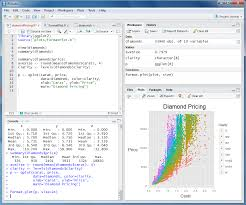
\includegraphics[width=0.6\linewidth]{rstudio2}
\end{figure}



%----------------------------------------------------------%
\newpage
\subsection*{Question 2}

 
Why are we using \texttt{R} for the course track? Select all that apply. 


\begin{itemize}

\item[(i)] \texttt{R} is free. 

\item[(ii)] \texttt{R} has a nice IDE, Rstudio. 

\item[(iii)] \texttt{R} allows object oriented programming. 

\item[(iv)] \texttt{R} is the best cloud computing language. 

\end{itemize}

\begin{verbatim}
R Language Definition
http://cran.r-project.org/doc/manuals/r-release/R-lang.html
\end{verbatim}
%----------------------------------------------------------%
\newpage
\subsection*{Resource for Learning R}

% Using Help Files
% Intro to R
% Stack Overflow
% Rseek
% #Rstats
% DataCamp
% SWIRL

\begin{itemize}
\item  Using Help Files ( for example \texttt{ help(sort) })
\item Introduction to R ( command \texttt{help.start()} - top left of page)
\item Stack Overflow (stackoverflow.com)
\item Rseek.org
\item Using Twitter: \texttt{\#Rstats}
\item www.datacamp.com
\item SWIRL
\end{itemize}

%----------------------------------------------------------%
\newpage
%Learning Resources
\subsection*{Question 3}
 
What are good ways to find answers to questions in this course track? Select all that apply. 

\begin{itemize}

\item[(i)] Searching Google. 

\item[(ii)]  Posting homework assignments to mailing lists 

\item[(iii)] Looking through \texttt{R} help files. 

\item[(iv)] Expecting every answer to be in a lecture slide 
\end{itemize}

%----------------------------------------------------------%
\newpage
% Question 4
% Appropriate Behaviour
\subsection*{Question 4}

 
What are characteristics of good questions on the message boards? \\ Select all that apply.
 

\begin{itemize}

\item[(i)] Is polite and courteous. 

\item[(ii)] Provides no details. 

\item[(iii)] Explicitly lists versions of software being used. 

\item[(iv)] is insulting or rude. 
\end{itemize}


%----------------------------------------------------------%
\newpage
\subsection*{CRAN}
\begin{itemize}
\item The Comprehensive R Archive Network
\item http://cran.r-project.org/
\end{itemize}
\subsection*{Task views}


%----------------------------------------------------------%
\newpage
\subsection*{Question 5}

Which of the following packages provides Machine Learning Functionality
\begin{itemize}
\item[(i)] \textbf{\textit{knitr}}
\item[(ii)] \textbf{\textit{filehash}}
\item[(iii)] \textbf{\textit{gbm}}
\item[(iv)] \textbf{\textit{kernlab}}
\end{itemize}

%----------------------------------------------------------%
\newpage
\subsection*{Optional Exercise}
Following from Question 5, search the CRAN package repository to find a package 
related to each of the following topics.
\begin{enumerate}
\item Graphics
\item Biology
\item Archeology
\item Marine or Maritime Sciences
\item Medical Imaging
\item Missing Data
\item Quality Control
\item Social Sciences
\item Text Analytics
\end{enumerate}

%----------------------------------------------------------%
\newpage
\subsection*{Optional Exercise}

\textbf{10 packages every data scientist should know}


\end{document}


\subsection*{END HERE}








%--------------------------------------------------------------------%
Question 5
 
Which of the following packages provides machine learning functionality? Select all that apply
 

\item[(i)] knitr 

\item[(i)] filehash 

\item[(i)] gbm 

\item[(i)] kernlab 

%--------------------------------------------------------------------%


\subsection*{Question 1}
We take a random sample of individuals in a population and identify whether they smoke and if they have cancer. We observe that there is a strong relationship between whether a person in the sample smoked or not and whether they have lung cancer. 
\\
\\
We claim that the smoking is related to lung cancer in the larger population. We explain we think that the reason for this relationship is because cigarette smoke contains known carcinogens such as arsenic and benzene, which make cells in the lungs become cancerous.
\begin{itemize}
\item This is an example of a causal data analysis.
\item This is an example of a predictive data analysis.
\item This is an example of an inferential data analysis.
\item This is an example of a mechanistic data analysis.
\end{itemize}
\newpage
%-------------------------------------------%
\subsection*{Question 2}
What is the most important thing in Data Science?
\begin{itemize}
\item Statistical inference.
\item Machine learning and prediction.
\item The data.
\item The question you are trying to answer.
\end{itemize}

\newpage
\section*{The Data Scientist’s Toolbox - Week 2 Quiz}

%-----------------------------------------------------------------------------------%
\subsection*{Question 1}
Which of the following commands will create a directory called data in your current working directory?
\begin{itemize}
\item mkdir data
\item pwd ../data
\item pwd data
\item mkdir /Users/data
\end{itemize}
%-----------------------------------------------------------------------------------%
\subsection*{Question 2}
Which of the following will initiate a git repository locally?

\begin{itemize}
\item[(i)]  git merge origin master
\item[(ii)]  git push
\item[(iii)]  git boom
\item[(iv)]  git init
\end{itemize}
%-----------------------------------------------------------------------------------%
\subsection*{Question 3}
Suppose you have forked a repository called datascientist on Github but it isn't on your local computer yet. Which of the following is the command to bring the directory to your local computer? (For this question assume that your user name is username)

\begin{itemize}
\item[(i)] git pull datascientist master
\item[(ii)] git init
\item[(iii)] git push origin master
\item[(iv)] git clone https://github.com/username/datascientist.git
\end{itemize}
%-----------------------------------------------------------------------------------%
\subsection*{Question 4}
Which of the following will create a markdown document with a secondary heading saying "Data Science Specialization" and an unordered list with the following for bullet points: Uses R, Nine courses, Goes from raw data to data products
\begin{framed}
\begin{verbatim}
*h2 Data Science Specialization 

* Uses R 
* Nine courses 
* Goes from raw data to data products
\end{verbatim}
\end{framed}

\begin{framed}
\begin{verbatim}
## Data Science Specialization 

li Uses R 
li Nine courses 
li Goes from raw data to data products
\end{verbatim}
\end{framed}

\begin{framed}
\begin{verbatim}
*** Data Science Specialization 

* Uses R 
* Nine courses 
* Goes from raw data to data products
\end{verbatim}
\end{framed}

\begin{framed}
\begin{verbatim}
### Data Science Specialization 

* Uses R 
* Nine courses 
* Goes from raw data to data products
\end{verbatim}
\end{framed}

\begin{framed}
\begin{verbatim}
## Data Science Specialization 

* Uses R 
* Nine courses 
* Goes from raw data to data products
\end{verbatim}
\end{framed}
%-----------------------------------------------------------------------------------%
\subsection{Question 5}
Install and load the KernSmooth R package. What does the copyright message say?
\begin{itemize}
\item[(i)] Copyright M. P. Wand 1990-2009
\item[(ii)] Copyright M. P. Wand 1997-2009
\item[(iii)] Copyright Coursera 2009-2013
\item[(iv)] Copyright Matthew Wand 1997-2009
\end{itemize}

\newpage

\end{document}
